\subsection{Mechanisms}\label{sec:mech}
%\footnote{The analysis in this section is preliminary and the measure for desired occupations is currently refined.}
In this section we explore whether a particular type of occupations drive the $IVUR$ results. For this, we generate alternative measures of the $IVUR$. First, by desired occupations, which are usually registered by the caseworkers at the PES for each job-seeker. And second, by seasonal and non-seasonal jobs.
Additionally, we explore the concern, that the benefit cuts could be politically driven by controlling for the vote share intentions for the FPÖ (Freedom Party of Austria), a right-wing populist party.

\vspace{0.5cm}
\noindent\textbf{Labor demand by most desired occupations.}\hspace{0.5cm} A broad measure of labor demand reflects the overall situation of the local labor market. However, many jobs that firms are seeking to fill might not be accessible to refugees with short tenures in the host country due to a lack of necessary language skills or recognized qualifications. To investigate whether the occupations in demand matter, we use the detailed nature of the vacancy data to create alternative versions of the $IVUR$.

First, we create a measure of demand for occupations with particularly low entry barriers. The PES records \textit{desired occupations} for every person registering with the PES. Desired occupations are not necessarily the jobs a job seeker desires, but those that a caseworker considers realistic based on the job seeker’s prior experience and skills. We see a strong clustering for refugees, with four occupations accounting for more than 50\% of the desired occupations: construction, cleaning, cooking and kitchen assistance, and general manual labor. Thus, we consider labor demand in these four occupations.

Figure \ref{fig:occ_ivur} shows the effect of the $IVURs$ in desired occupations on employment and mobility. The impact of labor demand in desired occupations on employment is approximately three times larger than that of the overall measure (left figure). However, this effect is short-lived, diminishing sharply after 18 months. In contrast, mobility is also strongly affected in the short term, and the effects, while somewhat declining, persist over the 60-month observation period (right figure).\footnote{This analysis has two caveats. First, these jobs account for only a small fraction of all vacancies, and the regional variation in this $IVUR$ measure is significantly smaller. Thus, while the effect of labor demand in this occupation is large, the low variation implies that the overall effect of demand in these occupations on explaining mobility and employment differences between regions is small. Second, labor demand in these occupations might be correlated with labor demand in other occupations. In this case, the estimates would be upward-biased. To address this concern, we run a model that includes labor demand in all other but the desired occupations.
The estimated effect of demand in the other occupations is slightly smaller but similar to the main result. Desired occupations have a stronger but more short-lived effect on employment than other occupations. However, they account for only a small share of all occupations.
 % (not included in this version). 
}%, while the effect of $IPBL$ on employment is -0.051367, and on residing in the initial state is 0.09056.} 

\begin{figure}
    \caption{Effect of $IVUR$ in desired occupations on employment and mobility}
    \label{fig:occ_ivur}
    \begin{center}
    \vspace{-0.5 cm}
    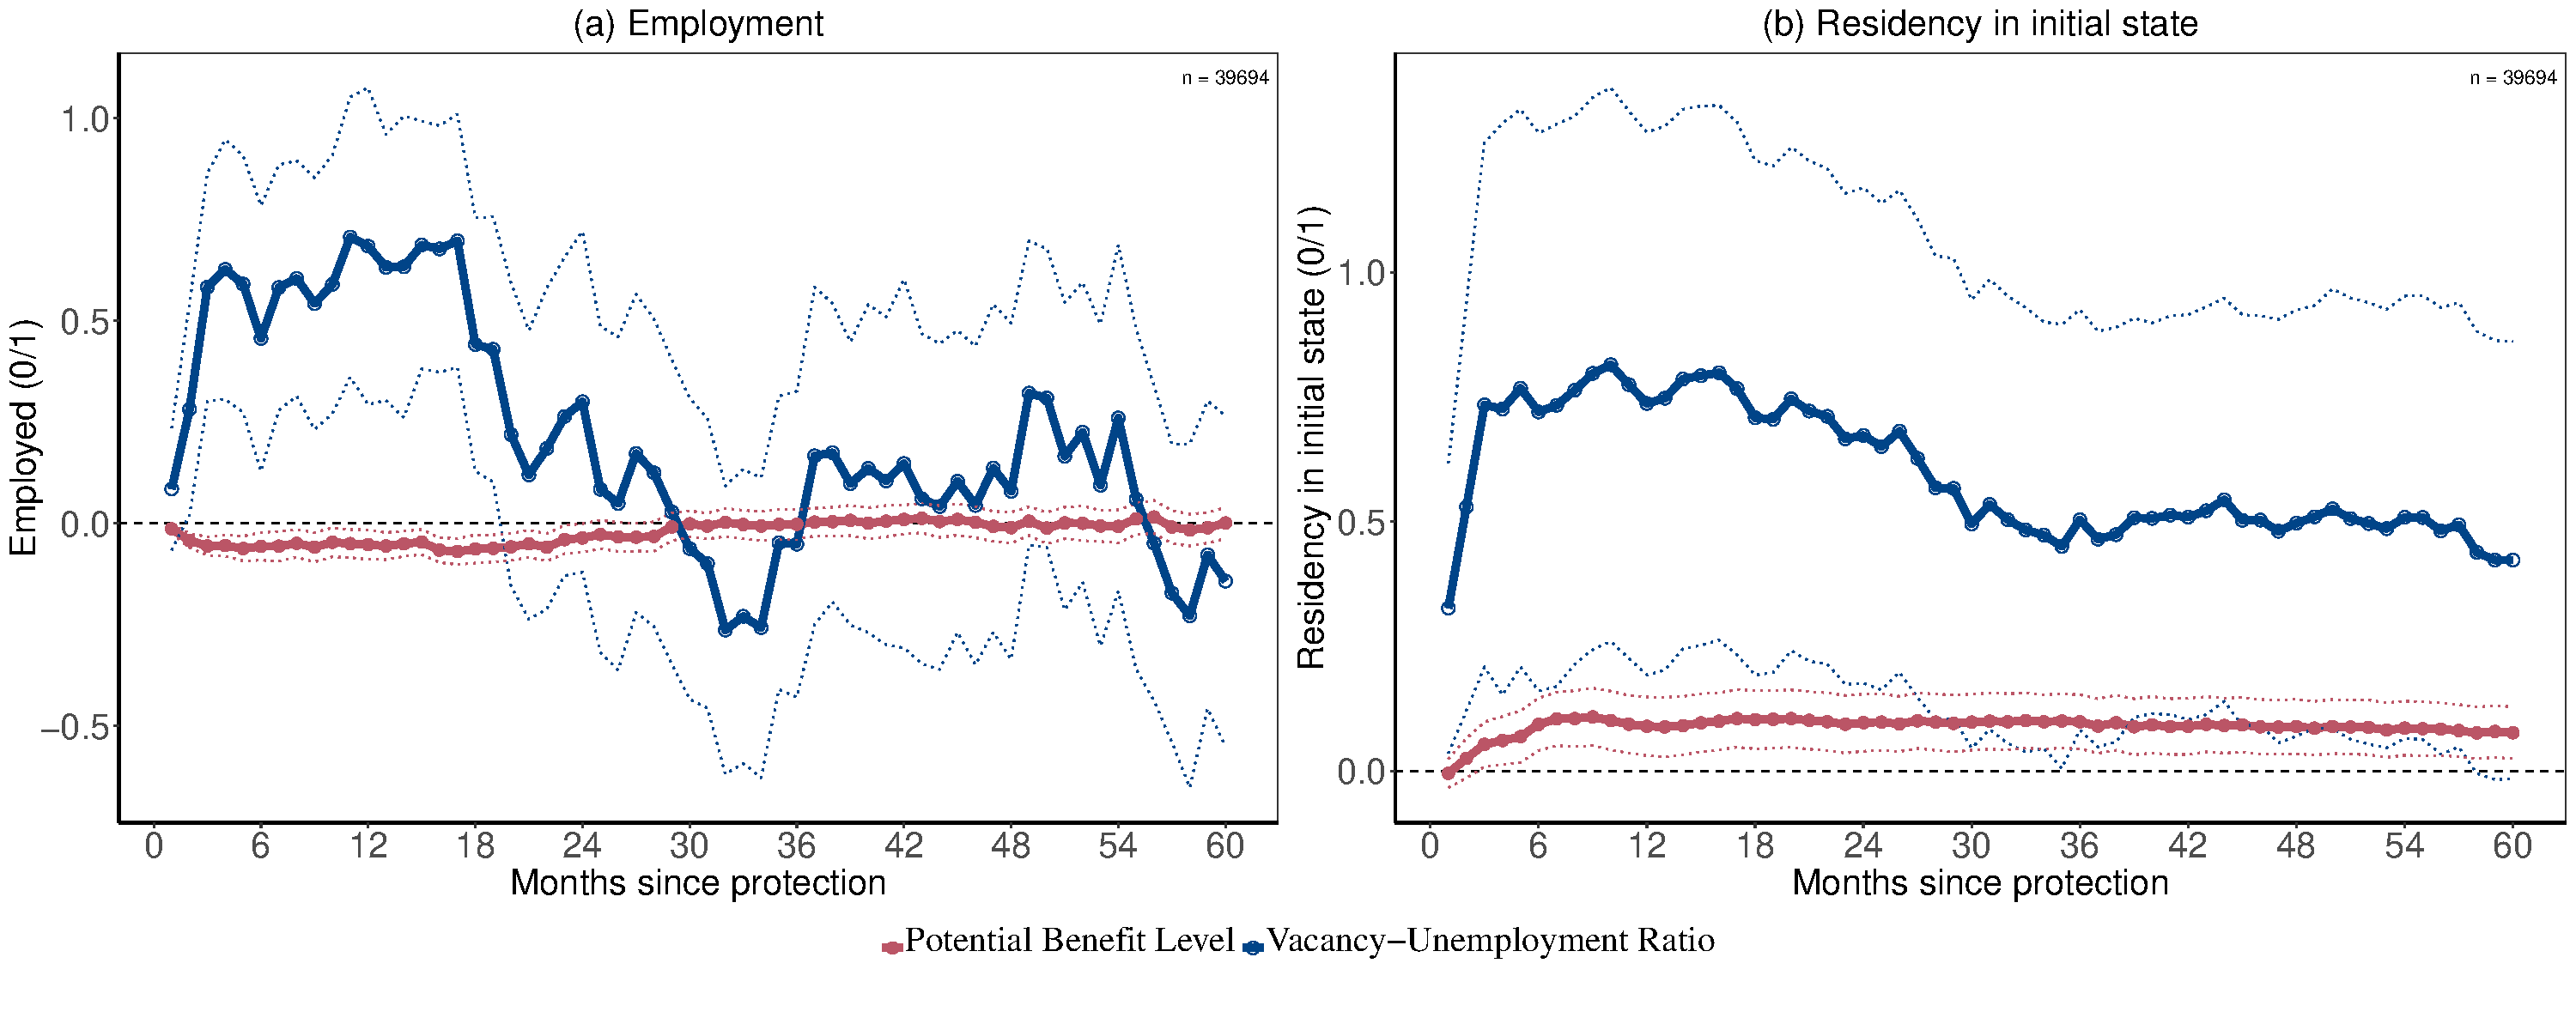
\includegraphics[scale=0.31]{figures/rob/fig_rob_labor_mobility_most_desired.pdf}
    \end{center}
    \vspace{-0.5cm}
    \fignote{\footnotesize \textit{Notes:} The x-axis shows the months since protection was received. The y-axis displays the effect of a one-unit increase in either i) the occupation-specific vacancy-to-unemployment ratio or ii) the potential benefit level, measured in €1,000 (real 2015 values), on employment (left) and mobility (right). All regressions include a full set of arrival-group, year-month, and district-of-protection fixed effects. Additional control variables include age and age squared at immigration, gender, type of protection, family status at protection date, and country of origin. Standard errors are clustered at the state-year-of-protection level.}
\end{figure}


\vspace{0.5cm}
\noindent\textbf{Labor demand by seasonal occupations.}\hspace{0.5cm} We create a measure for demand in jobs labeled as seasonal occupations, often found in the tourism industry. These jobs are of particular interest as they reflect truly short-term opportunities rather than long-term economic perspectives.

For both types of occupations, we create measures for the $IVUR$ by dividing the number of open positions in the respective categories by the number of job seekers. Note that we do not restrict job seekers to those looking in these specific occupations, as they often search in a broader range of fields.

\begin{figure}
    \caption{Effect of $IVUR$ in seasonal occupations on employment and mobility}
    \label{fig:seasonal_ivur}
    \begin{center}
    \vspace{-0.5 cm}
    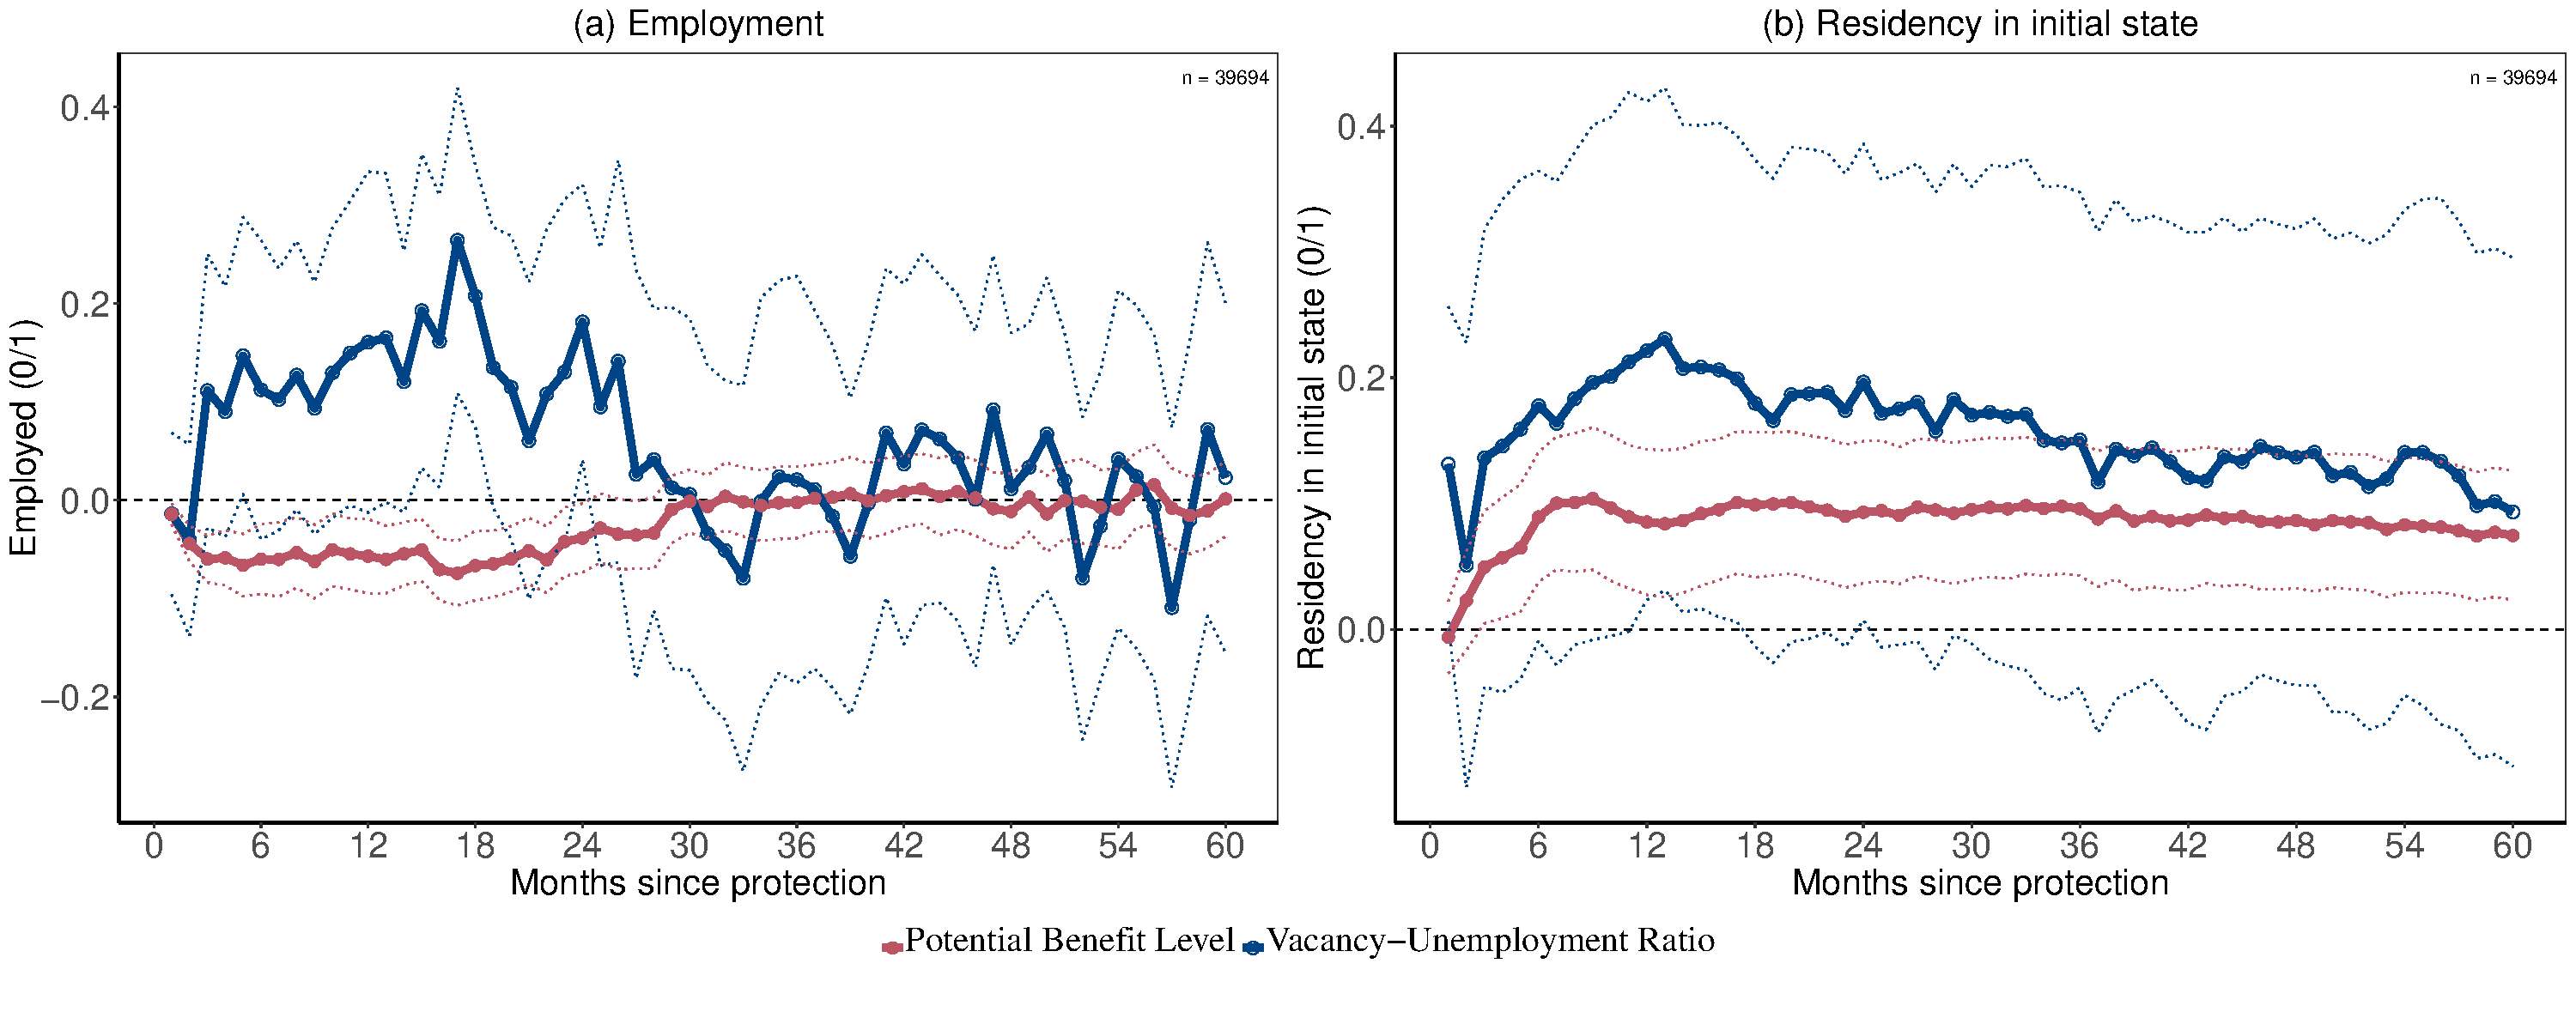
\includegraphics[scale=0.31]{figures/rob/fig_rob_labor_mobility_seasonal.pdf}
    \end{center}
    \fignote{\footnotesize \textit{Notes:} The x-axis shows the months since protection was received. The y-axis displays the effect of a one-unit increase in either i) the occupation-specific vacancy-to-unemployment ratio or ii) the potential benefit level, measured in €1,000 (real 2015 values), on employment (left) and mobility (right). All regressions include a full set of arrival-group, year-month, and district-of-protection fixed effects. Additional control variables include age and age squared at immigration, gender, type of protection, family status at protection date, and country of origin. Standard errors are clustered at the state-year-of-protection level.}
\end{figure}

Figure \ref{fig:seasonal_ivur} shows the effects of labor demand in seasonal occupations, Figure \ref{fig:non_seasonal_ivur} for the non-seasonal occupations. It is important to note that due to district-fixed effects, this demand does not reflect differences in the regional economic structure, such as tourist areas. Instead, it reflects pure short-term demand for labor due to likely idiosyncratic reasons. For example, certain weather conditions might increase or decrease labor demand in the tourist industry or agriculture at specific times \citep{baumgartner2023}. The demand for these seasonal occupations should thus not influence forward-looking decisions based on expected labor market chances. Nevertheless, we find that seasonal labor demand increases the likelihood of employment and persistently increases the likelihood of staying, with the effects being only slightly smaller than for non-seasonal occupations. 

Together, these results indicate that refugees' decisions are driven by immediate constraints rather than long-term considerations. The immediate opportunities provided by these jobs facilitate the difficult transition from refugee shelters to independent housing. Once refugees have transitioned, they are more likely to remain in their original location. However, these initial job opportunities do not set refugees on a different career track with long-term implications.

\begin{figure}
    \caption{Effect of the $IVUR$ for non-seasonal occupations and $IPBL$ on employment and location choice}
    \label{fig:non_seasonal_ivur}
    \begin{center}
    \vspace{-0.5 cm}
    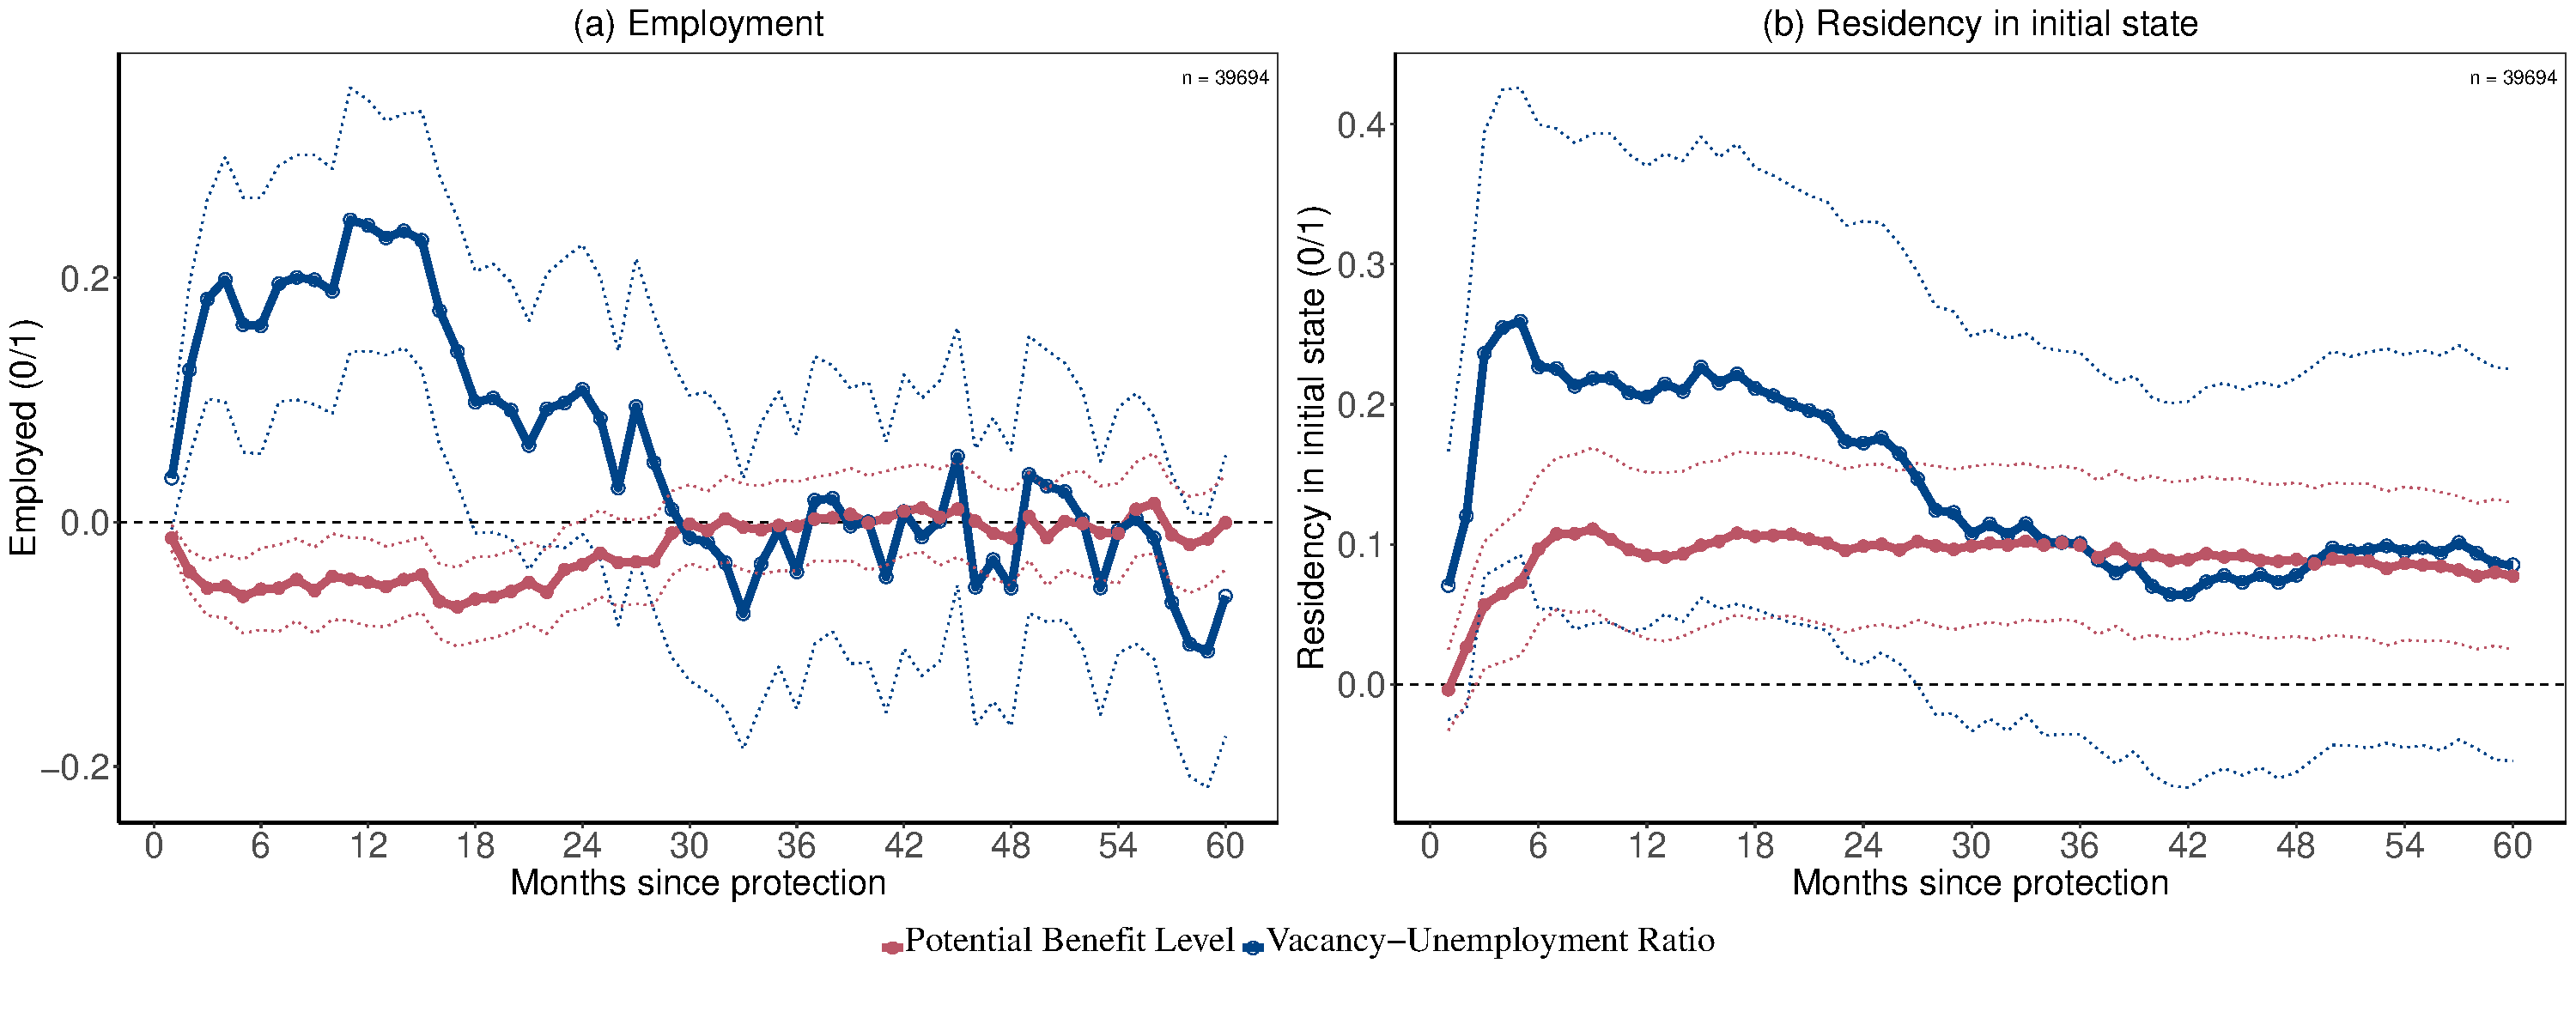
\includegraphics[scale=0.31]{figures/rob/fig_rob_labor_mobility_non_seasonal.pdf}
    \end{center}
    \fignote{\footnotesize \textit{Notes:} The x-axis shows the months since protection was received. The y-axis displays the effect of a one-unit increase in either i) the occupation-specific vacancy-to-unemployment ratio or ii) the potential benefit level, measured in €1,000 (real 2015 values), on employment (left) and mobility (right). All regressions include a full set of arrival-group, year-month, and district-of-protection fixed effects. Additional control variables include age and age squared at immigration, gender, type of protection, family status at protection date, and country of origin. Standard errors are clustered at the state-year-of-protection level.}
\end{figure}





\vspace{0.5cm}
\noindent\textbf{Comparison with concurrent single-sector studies.}\hspace{0.5cm} Two concurrent papers exploit the same Austrian dispersal setting but focus on single labor-market segments. \citet{degenhardt2025initial}, exploiting within-region, within-year seasonal variation in a hospitality-sector vacancy-to-unemployment ratio, finds an initial employment gain of up to 3 percentage points that diminishes after the first year, alongside positive cumulative earnings over three years and increased labor market segregation---complementary to our seasonal-occupations analysis above. \citet{degenhardt2025} use the geographic expansion of online food delivery firms as a low-barrier work treatment, finding that gig availability accelerates initial job-finding but traps workers in low-paid, unstable jobs, with negative effects on human capital and job search. Our general $IVUR$ measure nests these sectoral exercises in a single framework, finds a similar qualitative pattern with a longer fade horizon (around 30 months), and additionally jointly identifies the role of welfare benefit generosity.

\vspace{0.5cm}
\noindent\textbf{Benefit cuts and political decisions as confounder.}\hspace{0.5cm}
In our analysis, we exploit variation in benefit levels across states and refugee types (i.e., singles vs. families). One potential concern is that these benefit cuts may result from political decisions. For instance, more immigration-skeptical parties might attempt to reduce perceived "pull factors" by reducing benefit levels. If this is the case, then political decisions or ideology would be confounding our results and the effects of $IPBL$ would be upward-biased. 

To address this concern, we control for political sentiment using state-level voting intentions for the FPÖ---a far-right populist party---measured at the time of asylum approval. We gathered information on the voting intentions for the FPÖ from various polls as a proxy for the political sentiment in the states at the time when refugees received labor market access.

Figure \ref{fig:fpo} shows the results. Including the FPÖ vote share intentions as a control does not significantly affect the effects of $IPBL$ on employment and mobility.
However, the estimated effect of $IVUR$ on remaining in the initial state is halved compared to our main specification. This suggests that political sentiment might be a bad control for $IVUR$. If labor demand affects political preferences, then the FPÖ vote shares may themselves directly be affected by our variable of interest $IVUR$. 


\begin{figure}
    \caption{Robustness: Controlling for FPÖ Vote Share at Asylum Approval}
    \label{fig:fpo}
    \begin{center}
    \vspace{-0.5 cm}
    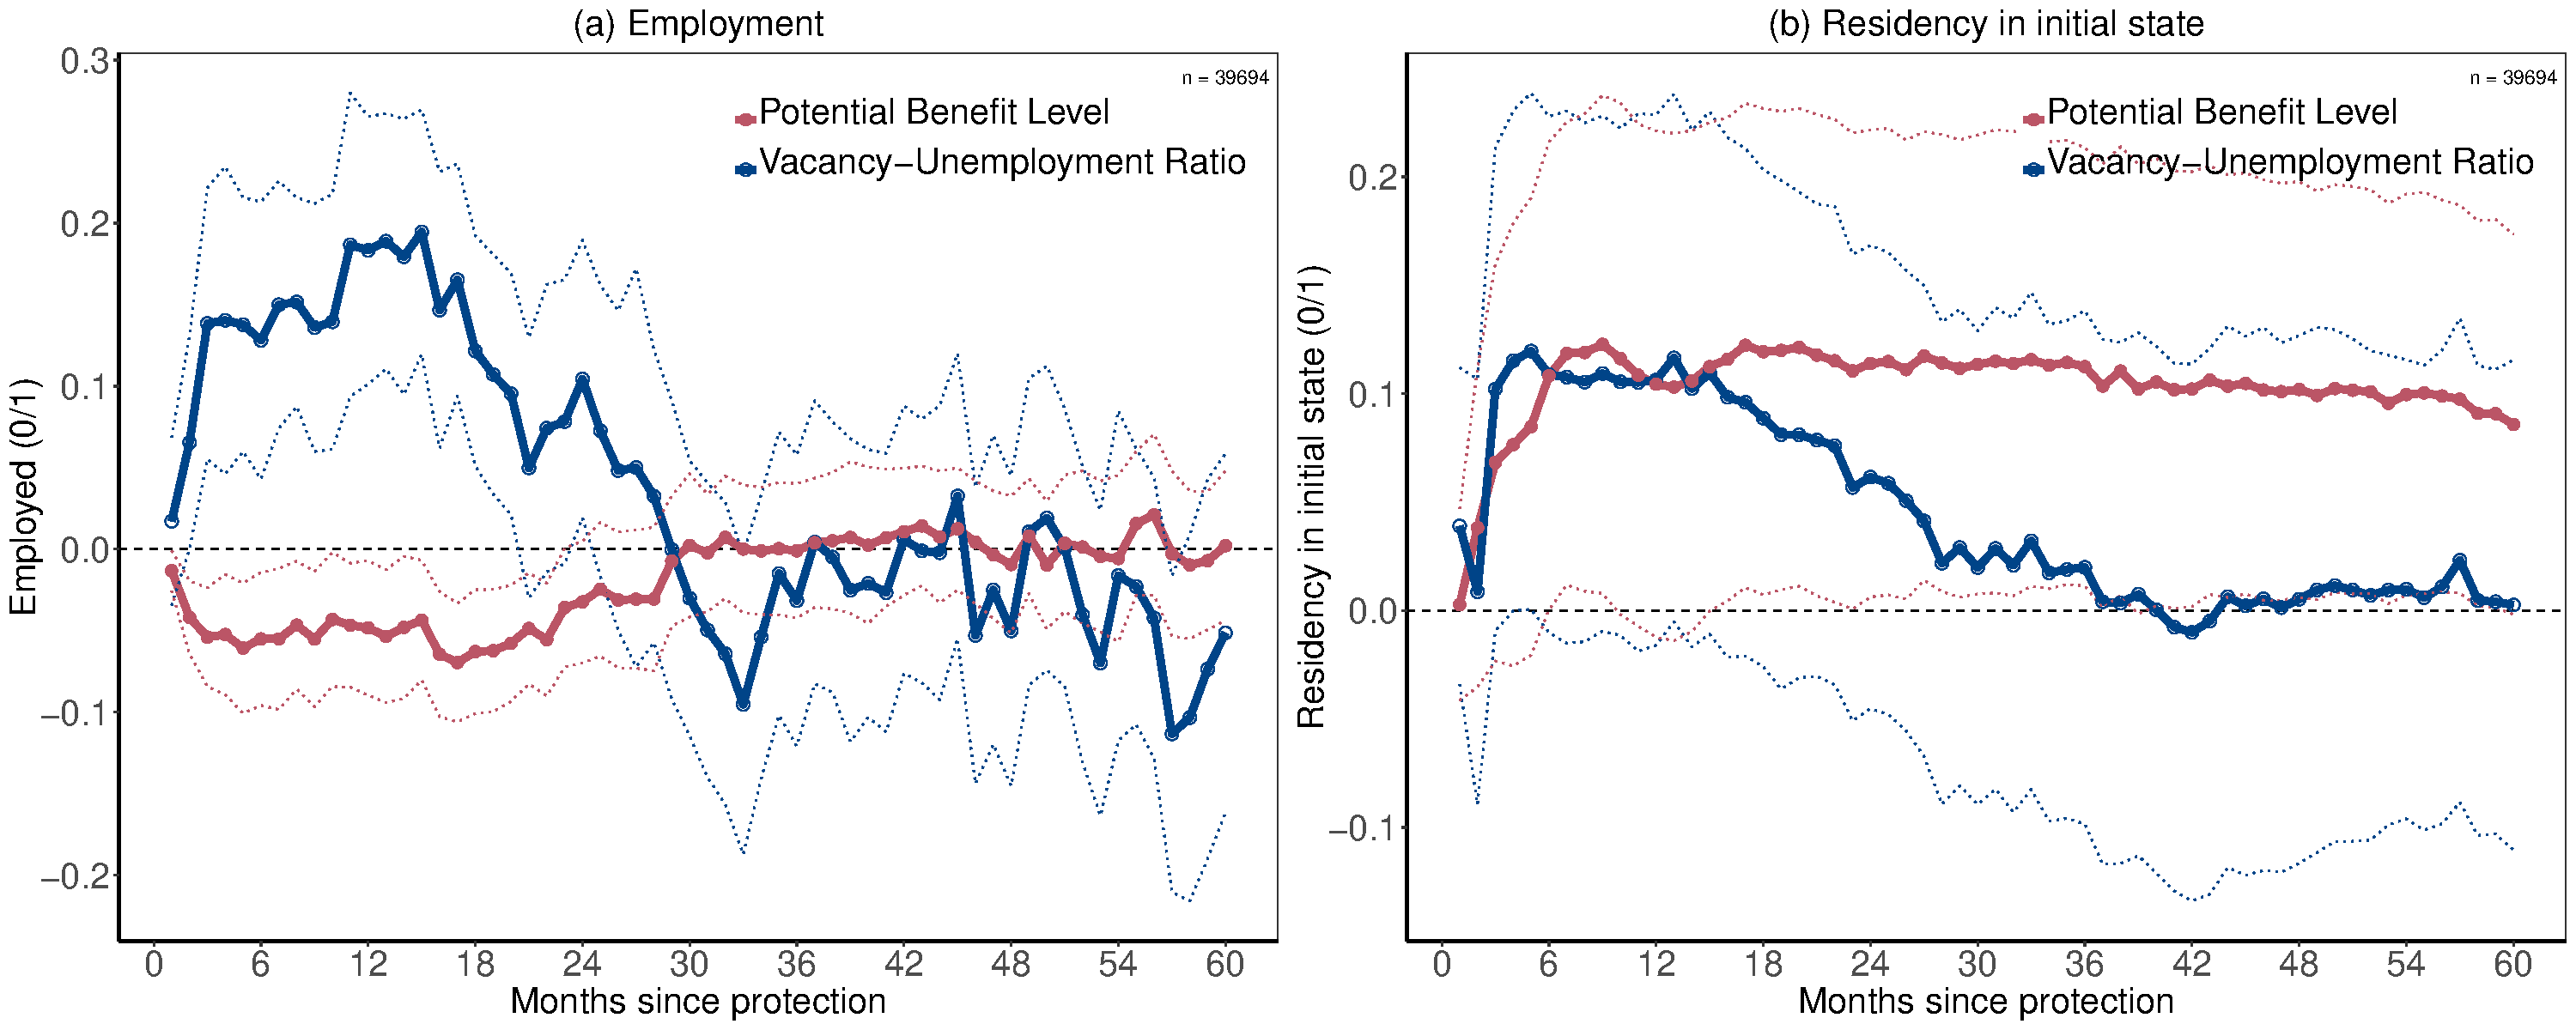
\includegraphics[scale=0.31]{figures/rob/fig_fp_share.pdf}
    \end{center}
    \vspace{-0.5 cm}
    \fignote{\footnotesize \textit{Notes:} The x-axis shows the months since protection was received. The y-axis displays the effect of a one-unit increase in either i) the vacancy-to-unemployment ratio or ii) the potential benefit level, measured in €1,000 (real 2015 values), on selected outcomes. The panels show the effects on (a) having any part- or full-time employment (binary) and (b) on the probability of living in the state of protection. All regressions include a full set of fixed effects for arrival group, year-month, and district of protection. Additional control variables include the FPÖ vote share at the state level at the time of protection, age and age squared at immigration, gender, type of protection, family status at protection date, and country of origin. Standard errors are clustered at the state-year-of-protection level. Dashed lines indicate 95\% confidence intervals.}
\end{figure}
